% Chapter 1 (from pres-main tex file)
% New Trends in Research
% Author: Javier Reyes

\subsection{DAEbot Project}

\begin{frame}
	\frametitle{DAEbot Project}
	\begin{columns}
		\begin{column}{0.4\textwidth}
			\begin{flushleft}
				\setstretch{1.5}\LARGE
				\textbf{D}istributed \\
				\textbf{A}rchitecture \\
				\textbf{E}valuation \\
				ro\textbf{BOT}
			\end{flushleft}
		\end{column} \pause
		\begin{column}{0.6\textwidth}
			\begin{figure}
				\includegraphics[width=\textwidth]{daebot-pic.png}
				\caption{DAEbot physical chasis.}\label{fig:daebot-pic}
			\end{figure}
		\end{column}
	\end{columns}
\end{frame}

\begin{frame}
	\frametitle{DAEbot Project}
	Characteristics\footnote[frame]{See oficial Wiki \cite{Wiki}}: \pause
	\begin{itemize}
		\item Designed to be modular.
		\item Allows different approaches for distributed HW and SW architectures. \pause
		\item Robust and big enough to carry several sensors and actuators.
	\end{itemize}
\end{frame}

\subsection{DAEbot Structure}

\begin{frame}
	\frametitle{DAEbot Structure}
	\begin{figure}
		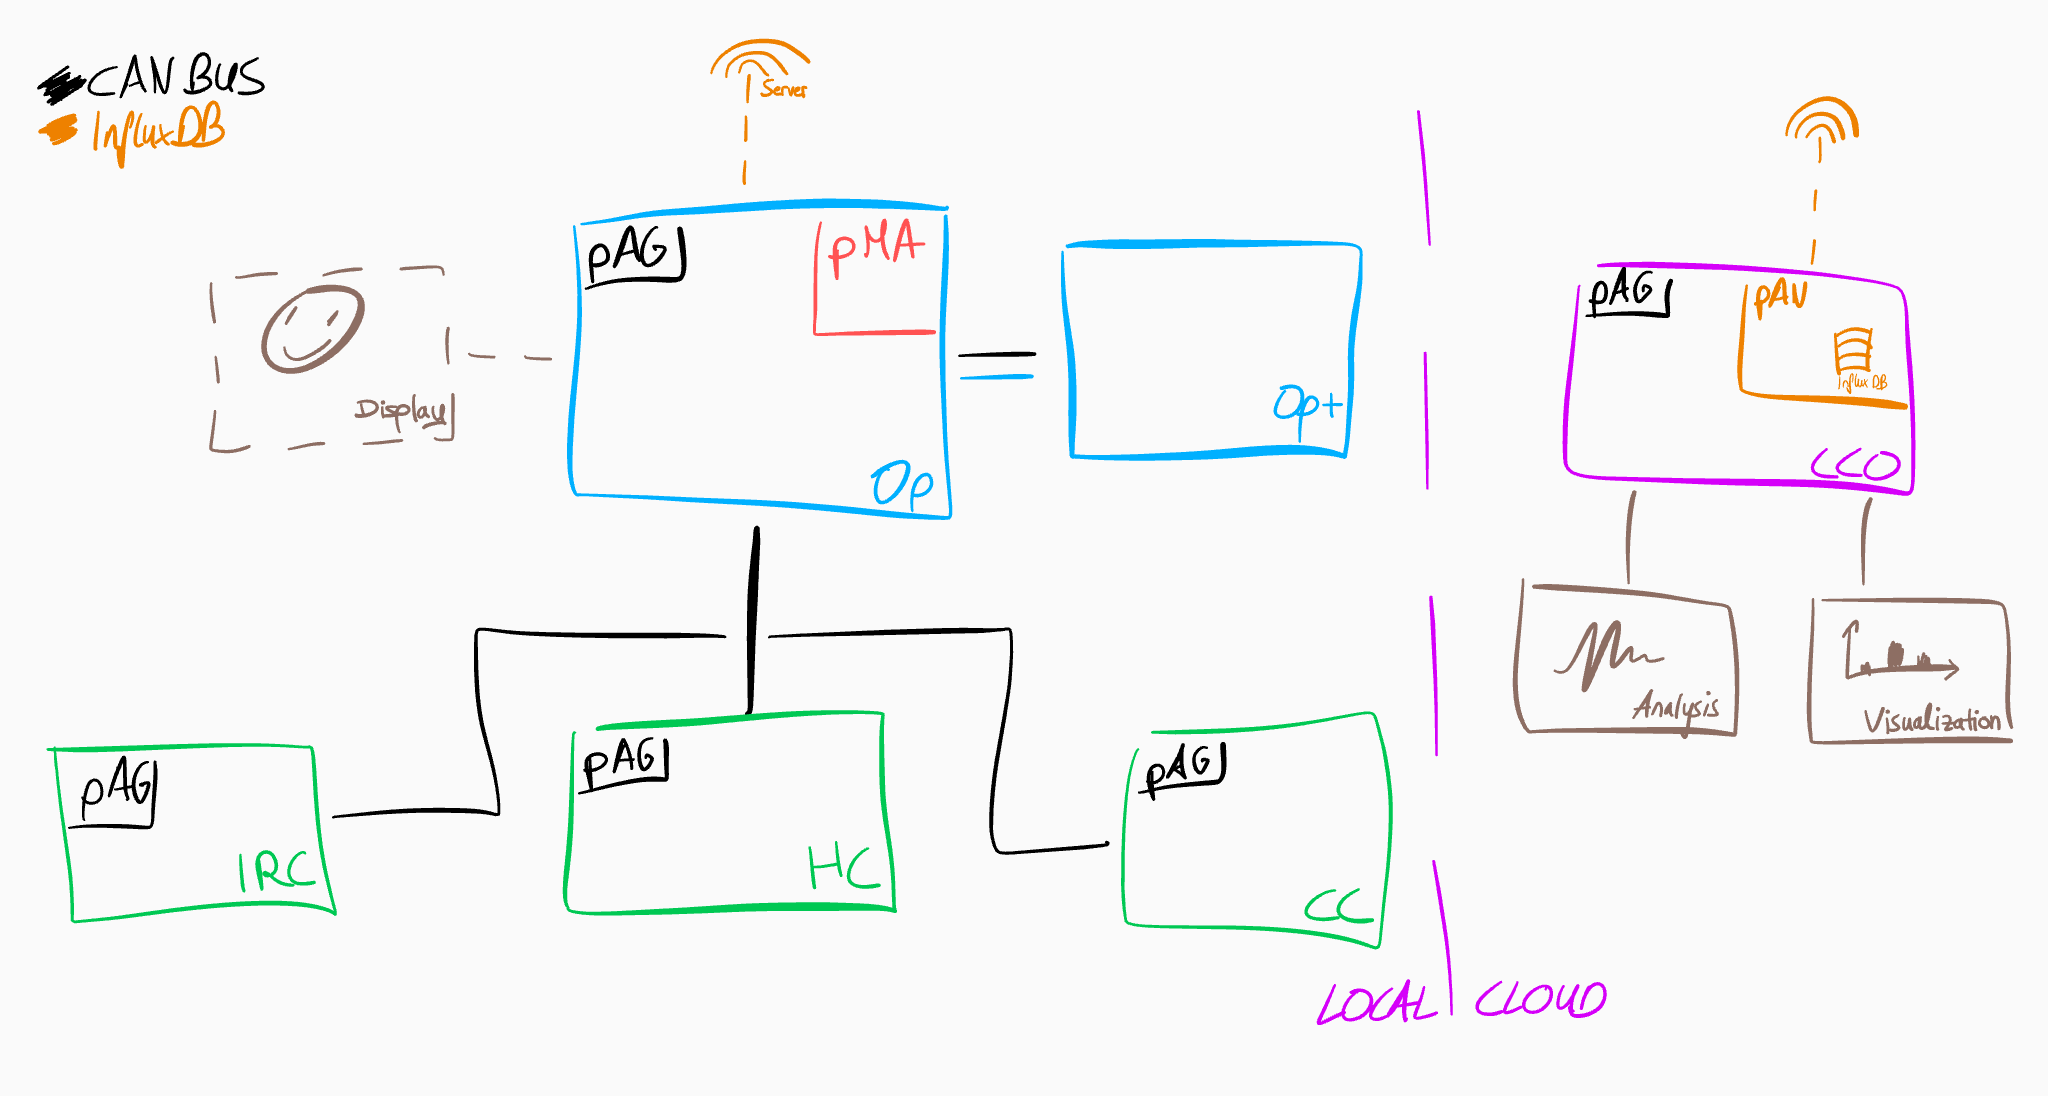
\includegraphics[width=0.7\textwidth, center]{daebot-concept-new.png}
		\caption{DAEbot software concept.}\label{fig:daebot-concept-new}
	\end{figure}
\end{frame}

\begin{frame}
	\frametitle{DAEbot Structure}
	\begin{figure}
		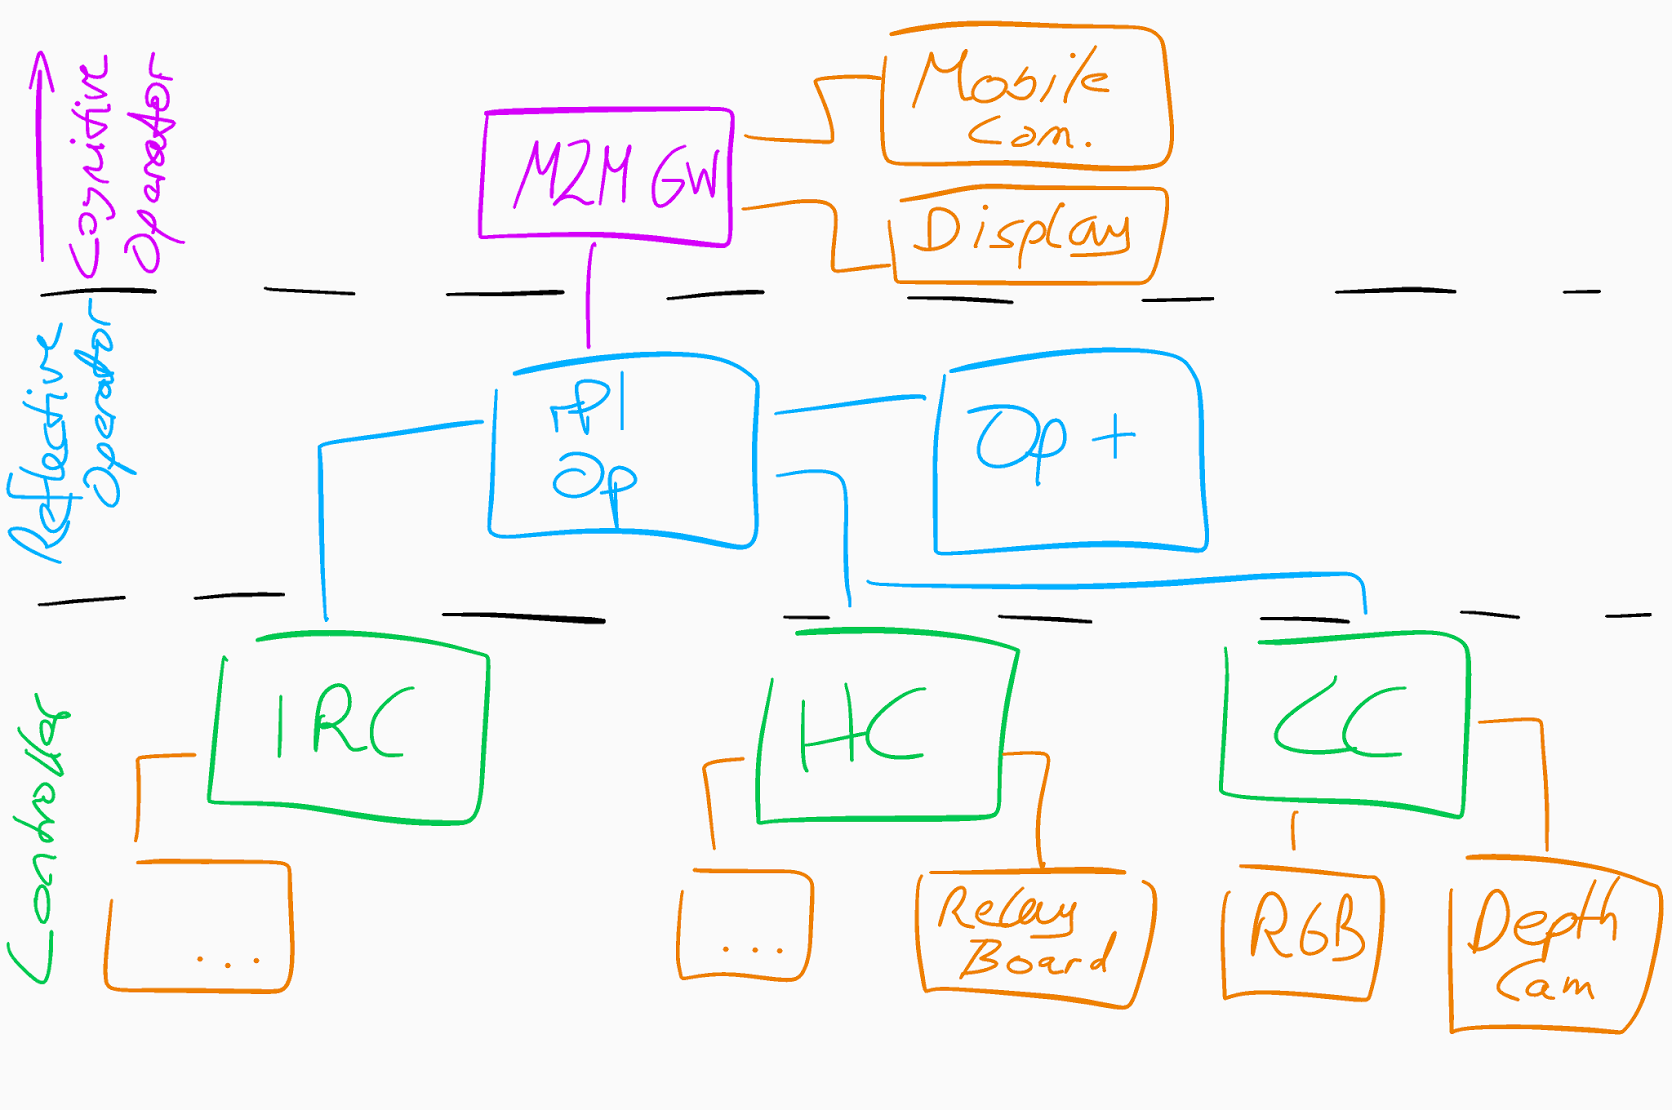
\includegraphics[width=0.7\textwidth, center]{daebot-concept-hand.png}
		\caption{DAEbot architecture, based on OCM concept.}\label{fig:daebot-concept-hand}
	\end{figure}
\end{frame}

\subsection{OCM Structure}

\begin{frame}
	\frametitle{OCM Structure}
	Layers\footnote[frame]{See \cite{Lueckel2001}}: \pause
	\begin{itemize}
		\item Controller: Lowest level layer, traditional controller as a \underline{control loop}, usually based on mathematical model. \pause
		\item Reflective Operator: Monitoring and control, allows communication with other systems in a network. \pause
		\item Cognitive Operator: Coordination/communication interactions or learning algorithms, expanded functionality.
	\end{itemize}
\end{frame}

\begin{frame}
	\frametitle{OCM Structure}
	\begin{figure}
		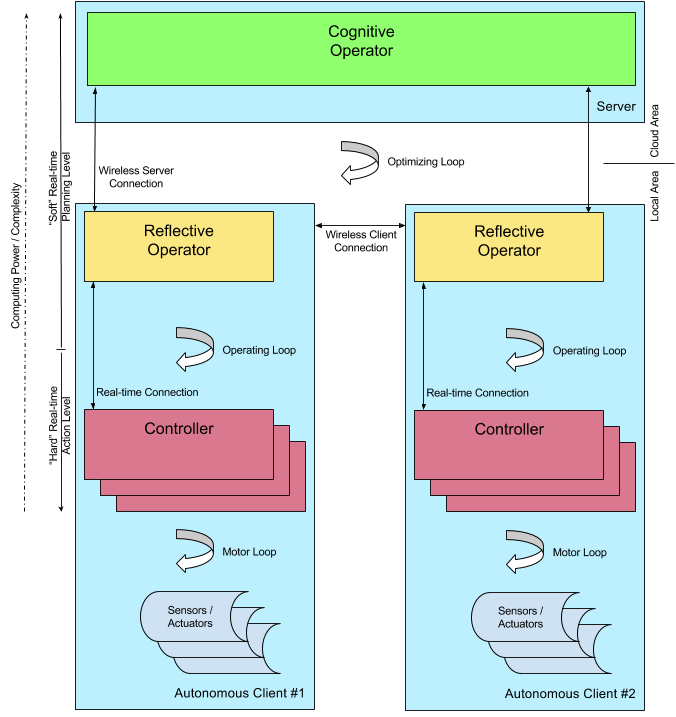
\includegraphics[width=0.5\textwidth, center]{ocm-architecture.png}
		\caption{OCM general structure diagram.}\label{fig:ocm-architecture}
	\end{figure}
\end{frame}

\begin{frame}
	\frametitle{DAEbot need}
	\textbf{\LARGE{Operator+ Goal:}} \\
	\large{Provide additional resources for the main Reflective Operator, thanks to its advantages in speed for parallel tasks in FPGA hardware.}
	\vfill \pause
	\begin{exampleblock}{Condition}
		The main Reflective Operator activates (via relay) the Operator+ when it is needed.
	\end{exampleblock}
\end{frame}